\chapter{Discussion}\label{ch:discussion}

The Results give three findings of different weight. Hydrogen exsolution releases a large heat
per kilogram, and the simulated excess enthalpies constrain it. Homogeneous nucleation keeps
exsolution close to equilibrium, so the metastable window of the published fit is not reached.
The source data constrain the heat, but they do not fix the spinodal. This chapter discusses
each finding and then the data that would sharpen them.

\section{What Sets the Heat of Exsolution}\label{sec:heat_discussion}

The heat follows from the excess enthalpy, which the homogeneous source simulations measure
directly \cite{gilmore2026data}. In refit M1, which matches the simulated enthalpies, it is
largest for dilute hydrogen, where each H$_2$ molecule is surrounded by silicate. The published
fit instead peaks near \pubThreshold{}\,wt\% (Section~\ref{sec:heat}). Below 1.2\,wt\%, the most
hydrogen-poor simulation, both are extrapolations. The binodal and the spinodal also depend on the
excess entropy and on the free energy inside the gap. The heat is therefore the better
constrained quantity: it depends on the enthalpy of homogeneous states, which the simulations
sample.

The published fit underestimates the simulated excess enthalpy of the most hydrogen-poor
mixture, \edHexPub{} against $\edHexData\pm\edHexSig$\,kJ\,mol$^{-1}$ (1$\sigma$), which is
\edHexPull{} standard deviations low. It overestimates the excess at $x = 0.83$. The refit M1 to
all data gives \edHexMOne{}\,kJ\,mol$^{-1}$ at $x = 0.24$. A refit to the phase compositions alone predicts
\edHexPhaseComp{}\,kJ\,mol$^{-1}$, which the enthalpy data exclude. A fit to phase data can thus
reproduce the gap with the wrong enthalpy. An evolution model that takes energies from a mixing
model, and not only phase boundaries, needs a model fitted to the enthalpies as well.

Two limits apply. First, the enthalpy data exist only at 4000\,K. The melt is reactive, and the
source simulations form hydroxyl, water and reduced silicon species \cite{gilmore2026}. Their
equilibria give an excess heat capacity, which all our model classes set to zero.
Section~\ref{sec:heat} estimates how much a plausible excess heat capacity changes the heat at
3000\,K. Second, near the critical point the hydrogen-rich phase is not pure H$_2$ and carries
silicate. Less heat is then released where hydrogen leaves the melt, and the rest follows higher
in the envelope as the silicate rains out \cite{tejada2026}. Our interior model sends the
exsolved hydrogen to pure H$_2$. It gives the total heat along the path, not where in the planet
that heat appears. Section~\ref{sec:interior} shows how much less heat the other end states
release at the top of the interior.

\section{Exsolution Heat and Planetary Cooling}\label{sec:cooling_discussion}

In a convecting interior the heat matters most while the top of the interior exsolves. Over the
first 300\,K below the binodal, the released heat is \intRatioThree{} times the sensible heat at
3\,wt\% (refit M1). Just below the binodal, exsolution adds up to \intGammaThree{} times the
sensible heat capacity (Section~\ref{sec:interior}). At a given heat flow, the top of the
interior therefore takes \intSlowThree{} times as long to cool through these 300\,K, and it
cools up to \intCeffThree{} times more slowly just below the binodal. At 1\,wt\% the ratio is
\intRatioOne{}, so the effect grows with the hydrogen content of the melt. These factors assume
that the hydrogen leaves as pure H$_2$, so they are upper bounds (Section~\ref{sec:interior}).

For the planet as a whole, the term is smaller. In the energy budget of Rogers et al.\
\cite{rogers2025}, gravitational contraction supplies most of the radiated energy. The sensible
heat of the interior is a minor term. Against that budget, the exsolution heat is
\planetRadiatedLo{}--\planetRadiatedHi{}\% of the energy radiated over 9\,Gyr and about
\planetThermal{} times the thermal-energy loss (Section~\ref{sec:interior}). If the planet kept
the same luminosity at each stage, the extra heat would lengthen its evolution by
\planetDelayLo{}--\planetDelayHi{}\% (published fit: \planetDelayPub{}\%; best-fitting refit:
\planetDelayMap{}\%). This estimate mixes two phase diagrams. The thermal history of Rogers et
al.\ uses the 2025 preprint fit \cite{stixrude2025}. Its binodal path stays above the 2026
critical temperature until about \planetCrossPubGyr{}\,Gyr, while our enthalpies come from the
2026 model. A consistent planetary
value needs an evolution model that takes the phase boundary and the heat from the same free
energy. None of the five evolution models we checked includes the heat of exsolution, either
explicitly or through a mixture equation of state
\cite{rogers2025,rogers2026,young2026,tang2026,tejada2026}. In the last of these, the mantle
holds no hydrogen.

\section{Exsolution Stays Close to Equilibrium}\label{sec:near_equilibrium}

Both routes to separation keep it close to the binodal. At the top of a convecting interior, the
melt touches the envelope, which is already the hydrogen-rich phase. Hydrogen can leave there
without nucleation. Deeper fluid is hotter and, because $T_C$ falls with pressure, further from
the gap. It enters the gap only when convection carries it to the top. Away from the envelope, a
parcel must nucleate the new phase. With the interface width of the simulated profile,
homogeneous nucleation ends metastability \dlyFigOneCPubLo{}--\dlyFigOneCPubHi{}\,K below the
binodal for the published fit and \dlyFigOneCMOneLo{}--\dlyFigOneCMOneHi{}\,K for refit M1. At
most \whFigOneCPubHi{}\% of the hydrogen is withheld (Section~\ref{sec:kinetics}). The wider
profile of a larger cell gives \dlyYoungPubLo{}--\dlyYoungPubHi{}\,K. Nucleation on interfaces,
such as crystals or droplets of an earlier-separated phase, can only shorten this delay
\cite{shea2017}.

The binodal--spinodal window of the published fit, \pubIntTwo{}\,K for this parcel, is therefore
a mean-field upper bound that a cooling parcel does not reach. Young et al.\ \cite{young2025}
plotted this window for the 2025 fit (their Fig.~2). Our calculation shows how far nucleation
falls short of it. Reaching half of the window would need an interface
\halfWinRatioLo{}--\halfWinRatioHi{} times wider than the simulated one
(Section~\ref{sec:kinetics}). The spinodal itself is a mean-field construct. For short-range forces, a sharp spinodal exists
only in mean-field theory \cite{klein1983}, and the crossover from nucleation to spinodal
decomposition is gradual \cite{binder1984}.

Three approximations limit these delays. The gradient coefficient comes from one simulated
profile in a small cell, which may include capillary broadening. Broadening makes the
coefficient and the delays too large, so removing it would shorten the delays further. How the
coefficient transfers between pressures matters for refit M1 but hardly for the published fit.
Matching the simulated width at 2\,GPa instead of 10\,GPa shortens the M1 delays about
threefold (two- to fivefold across the posterior) and the published-fit delays by 5--6\%. The
convention used here gives the longest delays.
% Typed: hand check with a separate script on 40 posterior samples (Appendix D).
The model uses one composition variable and one molar volume for both phases. Larger volumes
and longer times raise the nucleation criterion and shorten the delays further.

With near-equilibrium exsolution, the case for delayed hydrogen release largely disappears. A lag
would leave the envelope with less hydrogen than equilibrium predicts, not more. It would
therefore raise the mean molecular weight of the atmosphere for a while. In a convecting interior the top degasses
without delay, and an isolated parcel lags by at most \dlyFigOneCPubHi{}\,K for the simulated
interface width. Effects of a lag on the atmosphere are therefore negligible. A longer delay would need two conditions together. The
interior would have to be stratified in composition, so that fluid enters the gap without
touching the hydrogen-rich phase. And the nucleation barrier would have to be much larger than
the simulated interface implies.

\section{What the Source Data Can and Cannot Constrain}\label{sec:why}

The binodal and the spinodal probe different parts of the free energy. The binodal follows from
the common tangent, so it depends only on the free energy at the two coexisting compositions.
The spinodal depends on the curvature of the homogeneous free energy between them, a state that
phase-separated simulations do not sample. The perturbation of Section~\ref{sec:identifiability}
shows this for the present system. It changes the curvature inside the gap and leaves every bulk
equilibrium quantity unchanged. That bulk equilibrium fixes only the convex envelope of the free
energy is textbook thermodynamics. The perturbation is one admissible counterexample, so its
shifts are lower bounds on what the data leave open. With every heat capacity kept positive, it
moves the 3\,wt\% spinodal by only \bumpThree{}\,K. That is small against the M1 68\% range of
the baseline window, \IntMOneTableLo{}--\IntMOneTableHi{}\,K. It moves the 2\,wt\% spinodal,
near the cold end of the gap, by \bumpTwo{}\,K. At the baseline, the larger uncertainty comes
from the choice of functional form. The same limit applies to spinodals inferred from solubility data in other silicate--volatile
systems \cite{nishiwaki2025}.

Fitting a smooth model with few parameters ties the curvature inside the gap to the free energy
outside it. The spinodal is then as well constrained as these parameters, and three of them
matter together: the asymmetry $B/A$, the excess entropy set by $\tau$, and the strength of the
interaction. The source data pull them in different directions. Without the homogeneous data, the
fit returns to the published asymmetry ($B/A = \BAMOnePhaseComp{}$). The homogeneous enthalpies
favour a weak asymmetry ($B/A = \BAMOnePhaseHom{}$). None of our refits reproduces the published
combination. Their median windows span \IntRangeLo{}--\IntRangeHi{}\,K, against \pubIntTwo{}\,K
for the published fit. In mean-field theory, near the
critical point, the spinodal lies three times as far below $T_C$ as the binodal at the same
distance from $x_C$ \cite{debenedetti1996}. Near-critical data therefore constrain the spinodal
of near-critical parcels, but not of a parcel at $x = 0.435$. The runs most informative about the
curvature are also those whose compositions are least certain (Section~\ref{sec:audit}).

Two further effects bias the source data in ways that the posteriors do not include. First, the
coexistence runs use cells of 255--349 atoms with edges of 11--12\,\AA{} \cite{gilmore2026data}.
No size test exists for H$_2$--MgSiO$_3$, and Young et al.\ ran a single cell size
\cite{young2025}. The closest analogue is NH$_3$--H$_2$. There, cells of this size pull the
coexisting compositions toward the bulk by 0.1--0.2, and they converge only above about 8,000
atoms (\cite{gupta2026}, Fig.~S2). Correcting an inward bias of 0.05--0.10 per phase would raise
the best-fit $T_C$ at 2\,GPa by about 5--35\,K. It would change the 3\,wt\% window of the best
fit by $-50$ to $+45$\,K. A bias on the hydrogen-poor side narrows the window, and one on the
hydrogen-rich side widens it. A symmetric bias changes it by at most 15\,K.
% Typed: best-fit (MAP) refits of class M1 with shifted compositions, hand check on the
% current likelihood (Appendix D).
Cell size may also change whether a run near $T_C$ shows one phase or two, in either direction.
Wang, Hamel \& Cheng found H/He demixing temperatures about 2000\,K below earlier ab initio
studies with 64 atoms or fewer \cite{wang2026}. They name cell size as the likely main cause, by
ruling out other error sources, but they did not compute small-cell demixing temperatures. Their
result does not transfer to direct-coexistence runs. In their own structure-factor method, small
cells push toward mixing, which is the opposite sign.

Second, the runs are not strictly binary. In the coexistence runs the hydrogen-rich phase is
enriched in silicon, and near $T_C$ the tie lines lie well off the H$_2$--MgSiO$_3$ join
\cite{gilmore2026data}. Stability then requires the full composition Hessian to be
positive definite. Its smallest eigenvalue can vanish before the curvature along the
H$_2$--MgSiO$_3$ join does. For a given free energy, the binary spinodal is then a lower bound
in temperature. The binodal can move as well, so the sign of the change in the window is not fixed.

The excess volume adds a smaller caveat. The same group has simulated homogeneous
MgSiO$_3$H$_4$ with the same functional \cite{marcum2026}. These data put the excess volume at
5\,GPa and 4000\,K between $-1.4$ and $+0.2$\,cm$^3$\,mol$^{-1}$, smaller in magnitude than the
published $-1.78$\,cm$^3$\,mol$^{-1}$. Their smooth equation-of-state fit gives the published
value, but it misses their two 4000\,K points nearest 5\,GPa by about 11 and 26 standard
deviations in pressure.
% Typed: hand check on the data of Marcum et al. (2026), Appendix D.
They also find an excess volume that varies with pressure, which a constant $\pi$ cannot follow.
A $\pi$ fitted to the critical curve between 2 and 10\,GPa can then differ from the volume at
5\,GPa without any inconsistency in the data. The mismatch of Section~\ref{sec:audit} therefore
holds at one pressure and temperature, against the PBEsol endmembers of the source data.

\section{Data That Would Sharpen Both Results}\label{sec:design}

The cheapest improvement uses data that already exist. Per-run composition estimators, time
series and interface widths from the source authors would sharpen both results. The interface
widths fix the gradient coefficient, and with it the nucleation delay. The estimators and time
series fix the compositions of the near-critical runs, which drive $T_C$ and the spinodal. The
interfacial tension, from the stress anisotropy of the existing coexistence runs, would give an
independent value of the gradient coefficient. Homogeneous enthalpies below 4000\,K would test
the temperature dependence of the heat.

New simulations would narrow the spinodal only a little. A screen over candidate measurements
uses the posterior samples of the four model classes, each fitted to all data, with equal weight
(Figure~\ref{fig:design}). Consider one new homogeneous simulation at
$x \approx \designBestX{}$, with the precision of the existing ED Table~2 entries. It would
reduce the posterior standard deviation of the baseline spinodal only from \designSdNow{}\,K to
\designSdAfter{}\,K. The pooled spread has two main sources. The four model classes disagree on
the mean spinodal, and class M4 alone has a wide posterior. One more homogeneous point narrows
each class by only a few kelvin, so it removes neither source.

\begin{figure*}[t]
\centering
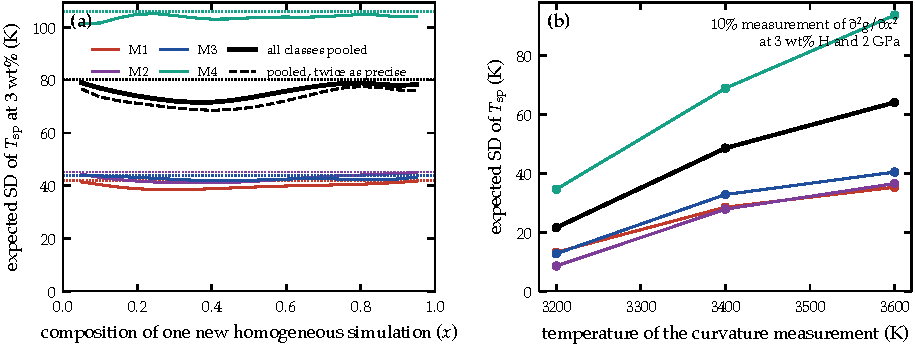
\includegraphics[width=\textwidth]{fig4_1_design}
\thesiscaption{Simulations that would constrain the spinodal.}{Expected posterior standard
deviation of the spinodal temperature of a 3\,wt\% parcel at 2\,GPa after (a) one new
homogeneous simulation of excess enthalpy, entropy and volume at composition $x$ with the
precision of the ED Table~2 entries, for each model class fitted to all data (thin lines) and
all classes pooled (thick line; dashed: pooled, twice that precision), with the current values
as dotted lines, and (b) a measurement of the composition curvature $\partial^2 g/\partial x^2$ at the baseline
composition with 10\% precision, at three temperatures. Linear-Gaussian screen of the
recalibration samples.}
\label{fig:design}
\end{figure*}

A direct measurement of the curvature does only slightly better. At 2\,GPa and \curvT{}\,K, a
10\% measurement of $\partial^2 g/\partial x^2$ at the baseline composition would reduce the
standard deviation from \designSdNow{}\,K to \curvSdPooled{}\,K. The screen covers 3200, 3400
and 3600\,K. Of these, \curvT{}\,K is the only temperature at which every posterior sample is
one phase (\curvFracOnePhase{}\%); at 3400\,K a single M4 sample is already two-phase. In a
one-phase parcel the simulation cannot decompose during the run. For the same reason, the
measured state lies outside the miscibility gap, where the perturbation of
Section~\ref{sec:identifiability} and its first two derivatives vanish. \curvT{}\,K is also above
the critical temperature of every sample and of the published fit (\pubTcTwo{}\,K), so no
composition at this temperature lies inside a gap. The measurement therefore cannot detect that
perturbation. It narrows the spinodal only through the functional forms of the four model
classes. The curvature follows from the long-wavelength
limit of the Bhatia--Thornton concentration--concentration structure factor,
$S_{cc}(0) = RT/(\partial^2 g/\partial x^2)$ per mole of mixing units \cite{bhatia1970,kirkwood1951}.
Four practical points apply. Simulations count atoms, not mixing units, so the normalisation must
be converted. The melt has several reacting species, so the full matrix of partial structure
factors is needed. At fixed particle numbers, $S_{cc}(0)$ requires an extrapolation to zero wave
number or a finite-volume Kirkwood--Buff correction \cite{kruger2013}. And the cell must be large.
Chen et al.\ state that structure-factor estimates of the curvature are nonnegative by
construction and limited by system size and run time \cite{chen2026}. They do not run a size
test. In
H/He, $S(0)$ converges only in cells of about 1700 atoms or more, roughly 14\,\AA{} across
(\cite{wang2026}, Supplementary Information). Present DFT-MD cells are smaller, so a machine-learned potential
trained on the same functional is the realistic route.
